\documentclass[12pt]{article}

%-------------PACKAGES------------- 
\usepackage[margin=1in]{geometry} 
\usepackage{amsmath,amsthm,amssymb}
\usepackage{pgfplots}
\usepackage{float}
\usepackage{braket}
\usepackage{titling}
\usepackage{wrapfig}
\usepackage{tikz}
\usepackage{mwe}
\usepackage{enumitem}
\usepackage{mathtools}
\usepackage{scrextend}
\usepackage{listings}
\usepackage{color}
\usepackage{caption}
\usepackage{subcaption}
\usepackage{algorithm,algpseudocode}
\usetikzlibrary{shapes,arrows,chains}
\usetikzlibrary[calc]

%-------------FORMATTING-------------
\setlength{\droptitle}{-7.5em} 
\setlength{\parindent}{0pt}
\def\LW{\dimexpr.25\linewidth-.5em} 
\tikzstyle{line} = [draw, -latex']

%--------------COMMANDS--------------
\newcommand{\N}{\mathbb{N}}
\newcommand{\Z}{\mathbb{Z}}
\newcommand{\R}{\mathbb{R}}
\newcommand{\C}{\mathbb{C}}
%\renewcommand{\qedsymbol}{\filledbox}

\DeclarePairedDelimiter \abs{\lvert}{\rvert}%
\DeclarePairedDelimiter \babs{\bigg\lvert}{\bigg\rvert}%
\DeclarePairedDelimiter \norm{\lVert}{\rVert}%

%------------ENVIRONMENTS------------- 
\newenvironment{theorem}[2][]{\begin{trivlist}
		\item[{\bfseries #1}\hskip \labelsep {\bfseries #2.}]}{\end{trivlist}}
\newenvironment{lemma}[2][Lemma]{\begin{trivlist}
		\item[\hskip \labelsep {\bfseries #1}\hskip \labelsep {\bfseries #2.}]}{\end{trivlist}}
\newenvironment{exercise}[2][Exercise]{\begin{trivlist}
		\item[\hskip \labelsep {\bfseries #1}\hskip \labelsep {\bfseries #2.}]}{\end{trivlist}}
\newenvironment{reflection}[2][Reflection]{\begin{trivlist}
		\item[\hskip \labelsep {\bfseries #1}\hskip \labelsep {\bfseries #2.}]}{\end{trivlist}}
\newenvironment{proposition}[2][Proposition]{\begin{trivlist}
		\item[\hskip \labelsep {\bfseries #1}\hskip \labelsep {\bfseries #2.}]}{\end{trivlist}}
\newenvironment{corollary}[2][Corollary]{\begin{trivlist}
		\item[\hskip \labelsep {\bfseries #1}\hskip \labelsep {\bfseries #2.}]}{\end{trivlist}}
\newenvironment{definition}[2][]{\begin{trivlist}
		\item[{\bfseries #1}\hskip \labelsep {\bfseries #2.}]}{\end{trivlist}}
\theoremstyle{remark}
\newtheorem*{remark}{Remark}

%-------------CODE-STYLE------------
\definecolor{dkgreen}{rgb}{0,0.6,0}
\definecolor{gray}{rgb}{0.5,0.5,0.5}
\definecolor{mauve}{rgb}{0.58,0,0.82}
\lstset{frame=tb,
	language=C++,
	aboveskip=3mm,
	belowskip=3mm,
	showstringspaces=false,
	columns=flexible,
	basicstyle={\small\ttfamily},
	numbers=none,
	numberstyle=\tiny\color{gray},
	keywordstyle=\color{blue},
	commentstyle=\color{dkgreen},
	stringstyle=\color{mauve},
	breaklines=true,
	breakatwhitespace=true,
	tabsize=3
}

\tikzset{
	path image/.style={
		path picture={
			\node at (path picture bounding box.center) {
				\includegraphics[height=3cm]{example-image}};}},
	path tikzimage/.style={
		path picture={
			\node at (path picture bounding box.center)
			[circle, fill=blue!50, scale=2, text=yellow]{Bravo};}}
}

\lstset{
	morekeywords={end}
}

%------------------------------------ 
%---------START-OF-DOCUMENT----------
%------------------------------------
\begin{document}
	
	\title{Paper Summary}
	\author{David Miller \\ 
		CIS 5930: Social Network Mining} 
	
	\maketitle 
	
	The advent of geo-tagged data has allowed computer scientists to implement a cariety of learning systems that involve taking a users location into account when learning and predicting. However current learning and predicting models have poor accuracy. The method proposed in this paper, \texttt{TRIOVECEVENT}, learns and predicts events with much higher results than those currently employed. At the very core of \texttt{TRIOVECEVENT} it mas ll the regions, times, and keywords into a latent space.. This is done via multimodal embedding where spatial, temporal, and textual units are mapped to lower-dimensional spaced with their correlations preserved. Mathematically we can describe the algorithm with the following notation. We let $\mathcal{D} = \{d_1, \dots, d_n, \dots\}$ be a continuous stream of tweets. Each tweet $d$ is a tuple $(t_d, l_d, x_d)$ where $t_d$ is its post time, $l_d$ is its location, and $x_d$ is a bag of keywords in the tweet. If we consider a query window $Q = [t_s, t_e]$ where $t_{d_1} \leq t_s < t_e \leq t_{d_n}$ the local event detection aims at extracting all local events that occur during $Q$ and updating the event list online as $Q$ shifts continuously \cite{paper}. A novel Bayesian mixture clustering model is used to divide the tweets in the query window $Q$ into a number of geo-topic clusters to generate candidates. Clusters contain tweets that are close in latent space due to there spatial and textual correlation. 
	\begin{wrapfigure}{r}{0.5\textwidth}
		\vspace{-15pt}
		\hspace{0pt}
		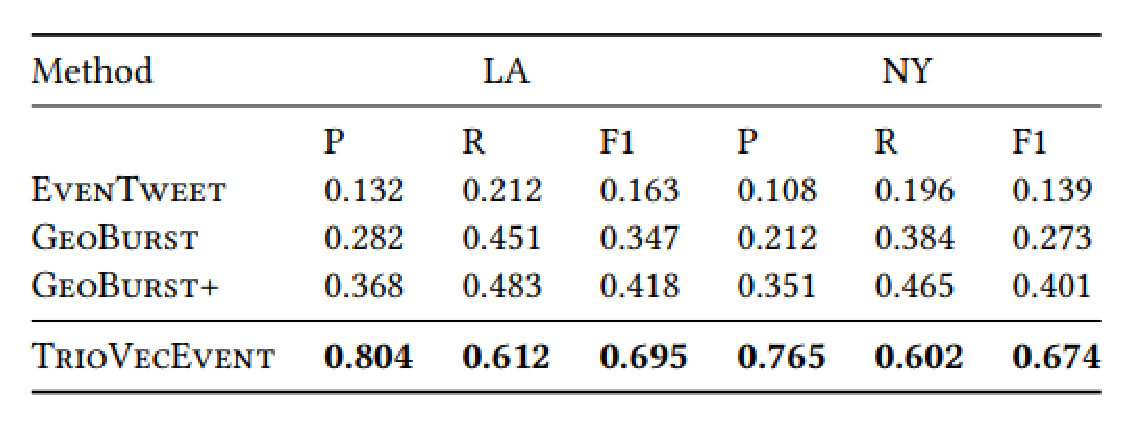
\includegraphics[height=3cm,width=0.5\textwidth]{fig1.eps}
		\caption{}
		\vspace{-14pt}
	\end{wrapfigure} 
	These candidates are then classified based on six properties: spatial unusualness, temporal unusualness, spatiotemproal unusualness, semantic concentration, spatial and temporal concentration, and burstiness. The results for this method are significantly better than other methods. Figure 1 shows the results of $\texttt{TRIOVECEVENT}$ vs two other methods; 'P' is precision and 'R' is pseudo recall. Evidently the \texttt{TRIOVECEVENT} outperforms its competitors. In terms of future work I feel like $\texttt{TRIOVECEVENT}$ should also be able to cluster events that are not just in one location, such as presidential elections or global movements. The latent space mapping will map these not too close to each other since their geo-location is not close. Another direction that can be taken is using this in disaster prevention technology. If \texttt{TRIOVECEVENT} can detect oncoming emergencies based on tweets, this can be incorporated in communities to detect them of oncoming dangers. \\
	
	Three strengths I found with the paper are
	\begin{enumerate}
		\item The noticeable gains in accuracy compared to other methods.
		\item The time complexity is linearly dependent on the number of new tweets.
		\item \texttt{TRIOVECEVENT} lends itself to a myriad of applications.
	\end{enumerate} 
	\vspace{0.5cm}
	
	Three weaknesses I found with the paper are
	\begin{enumerate}
		\item The paper only compared its results to two other methods, leading me to think there are methods that may come close to its accuracy.
		\item The paper makes no mention of using other social streams other than Twitter. This can lead to some bias due to Twitter's posting rules and the limit of tweets the API feeds you. Essentially the sample space may not be fully representative. 
		\item The algorithm relies on social data when in reality there are events that may not be allowed to be broadcast. Examples include countries or regions that impose restrictions on their citizens. 
	\end{enumerate}
	\vspace{0.5cm}
	
	Questions for the reader
	\begin{enumerate}
		\item How dos the model deal with spoofed locations, if at all?
		\item How does the model deal with multiple tweets from the same user?
	\end{enumerate}
	\vspace{0.5cm}
	
	\begin{thebibliography}{unsrt}
		\bibitem{paper}
		Chao Zhang, Liyuan Liu, Dongming Lei, Quan Yuan, Honglei Zhuang, Tim Hanratty, Jiawei Han \emph{TrioVecEvent: Embedding-Based Online Local Event Detection
			in Geo-Tagged Tweet Streams}, KDD’17, August 13-17, 2017, Halifax, NS, Canada.
	\end{thebibliography}
	
\end{document}\documentclass[12pt]{article}